% article example for classicthesis.sty
\documentclass[10pt,a4paper]{article} % KOMA-Script article scrartcl
\usepackage{lipsum}     %lorem ipsum text
\usepackage{titlesec}   %Section settings
\usepackage{titling}    %Title settings
\usepackage[margin=10em]{geometry}  %Adjusting margins
\usepackage{setspace}
\usepackage{listings}
\usepackage{amsmath}    %Display equations options
\usepackage{amssymb}    %More symbols
\usepackage{xcolor}     %Color settings
\usepackage{pagecolor}
\usepackage{mdframed}
\usepackage[spanish]{babel}
\usepackage[utf8]{inputenc}
\usepackage{longtable}
\usepackage{multicol}
\usepackage{graphicx}
\graphicspath{ {./Images/} }
\setlength{\columnsep}{1cm}

% ====| color de la pagina y del fondo |==== %
\pagecolor{black}
\color{white}



\begin{document}
    %========================{TITLE}====================%
    \title{\rmfamily\normalfont\spacedallcaps{ Apuntes analisis de datos clase 1 : Introduccion }}
    \author{\spacedlowsmallcaps{Rodrigo Castillo}}
    \date{\today} 
    
    \maketitle
     

     % ====| Loguito |==== %
    
\includegraphics[width=0.1\linewidth]{negro_cara.png}
    %=======================NOTES GOES HERE===================%
    \section{introduccion:}
       % ====| es un curso largo pero se le puede sacar provecho |==== %
        \begin{enumerate}
            \item {el curso es re denso} 
            \item {clases 3 dias a la seman} 
            \item {es un curso bonito} 
            \item {regresion multiple} 
            \item {clustering} 
            \item {clasificacion} 
        \end{enumerate}
        % ====| presentacion de asignatura |==== %
        \subsection{presentacion de asignatura}
            \begin{itemize}
                \item {3 creditos} 
                \item {lider es juan F} 
                \item {horas de consulta de 9-11} 
            \end{itemize}	
            % ====| temas |==== %
            \subsection{evaluacion}
                \\ 3parciales de 20 
                \\ 15   de quices 
                \\ 25   de proyectos
            \subsection{libro :}
                esta en el silabo 
                \\ 
            \section{calendario}
                hay un calendario super bonito en eaulas hecho por edwin
    \section{Tema}
        \subsection{presentacion de clasificacion por redes convolucionales}
            ya hice un curso de redes convolucionales, pero el profesor mostró
            una aplicación de clustering que él hizo en el curso con un
            profesor
        \subsection{media muestral}
            x_{k} = \frac{1}{n}\sum_{i=0}^{n}x_{jk} para $ k_1 . k_2 k k_3  $  
        \subsection{varias variables}
            supongamos que tenemos n pares de medidas sobre dos variables
            % ====| Poner imagen que no sé en donde guardé el pantallazo |==== %
        \subsection{consideracion}
            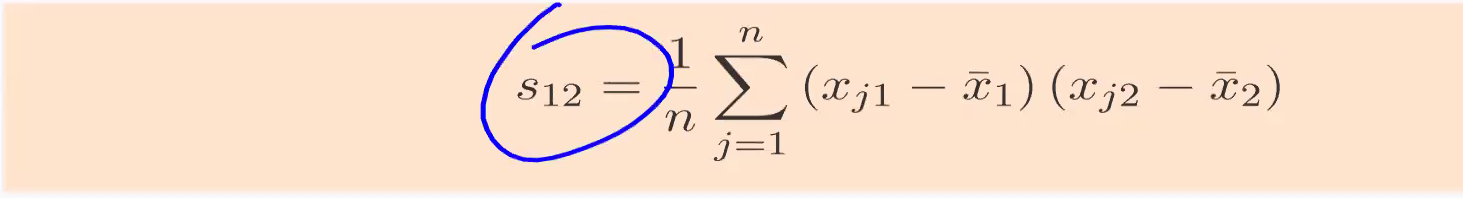
\includegraphics[width=0.8\linewidth]{cibsuderaciones.png}
            % ====| PONER CONSIDERACIONES DE LAS DIAPOSITIVAS |==== 
        \subsection{propuedades de las correlaciones}
            
            % ====| PONER PROPIEDADES DE LAS CORRELACIONES |==== %
        \section{estadistica descriptiva matricial}
            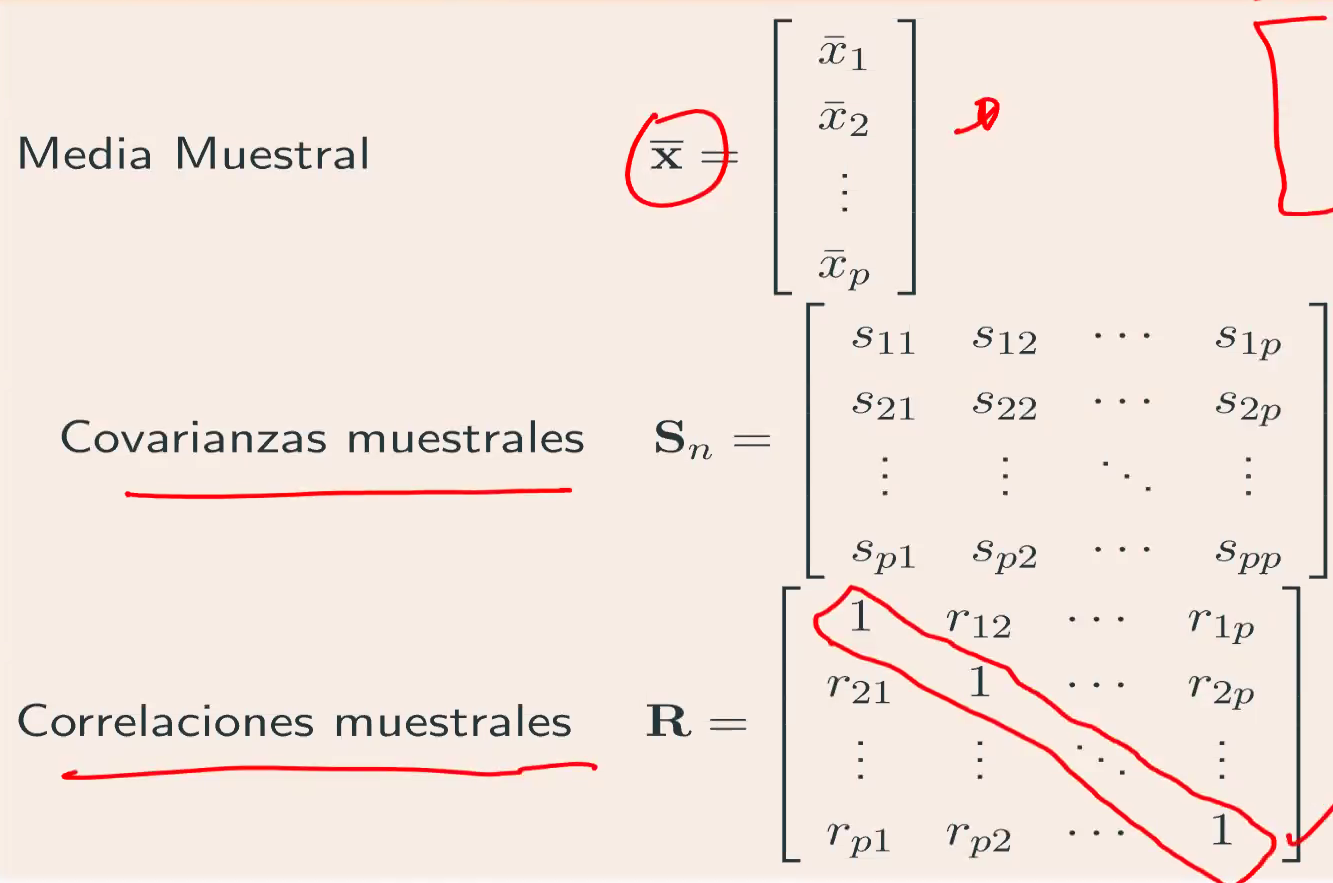
\includegraphics[width=0.8\linewidth]{propiedades.png}
            
            
                 
             
            
            
             
            
            
        
    







    %=======================NOTES ENDS HERE===================%
    
    % bib stuff
    \nocite{*}
    \addtocontents{toc}{\protect\vspace{\beforebibskip}}
    \addcontentsline{toc}{section}{\refname}    
    \bibliographystyle{plain}
    \bibliography{../Bibliography}
\end{document}
